%%%%%%%%%%%%%%%%%%%%%%%%
%% Sample use of the infthesis class to prepare a thesis. This can be used as 
%% a template to produce your own thesis.
%%
%% The title, abstract and so on are taken from Martin Reddy's csthesis class
%% documentation.
%%
%% MEF, October 2002
%%%%%%%%%%%%%%%%%%%%%%%%

%%%%
%% Load the class. Put any options that you want here (see the documentation
%% for the list of options). The following are samples for each type of
%% thesis:
%%
%% Note: you can also specify any of the following options:
%%  logo: put a University of Edinburgh logo onto the title page
%%  frontabs: put the abstract onto the title page
%%  deptreport: produce a title page that fits into a Computer Science
%%      departmental cover [not sure if this actually works]
%%  singlespacing, fullspacing, doublespacing: choose line spacing
%%  oneside, twoside: specify a one-sided or two-sided thesis
%%  10pt, 11pt, 12pt: choose a font size
%%  centrechapter, leftchapter, rightchapter: alignment of chapter headings
%%  sansheadings, normalheadings: headings and captions in sans-serif
%%      (default) or in the same font as the rest of the thesis
%%  [no]listsintoc: put list of figures/tables in table of contents (default:
%%      not)
%%  romanprepages, plainprepages: number the preliminary pages with Roman
%%      numerals (default) or consecutively with the rest of the thesis
%%  parskip: don't indent paragraphs, put a blank line between instead
%%  abbrevs: define a list of useful abbreviations (see documentation)
%%  draft: produce a single-spaced, double-sided thesis with narrow margins
%%
%% For a PhD thesis -- you must also specify a research institute:
%\documentclass[phd,ilcc,twoside]{infthesis}

%% For an MPhil thesis -- also needs an institute
% \documentclass[mphil,ianc]{infthesis}

%% MSc by Research, which also needs an institute
% \documentclass[mscres,irr]{infthesis}

%% Taught MSc -- specify a particular degree instead. If none is specified,
%% "MSc in Informatics" is used.
\documentclass[msc,cs,twoside,openright,logo,rightchapter,normalheadings,notimes]{class/infthesis}
% \documentclass[msc]{infthesis}  % for the MSc in Informatics

%% Master of Informatics (5 year degree)
% \documentclass[minf]{infthesis}

%% Undergraduate project -- specify the degree course and project type
%% separately
% \documentclass[bsc]{infthesis}
% \course{Artificial Intelligence and Psychology}
% \project{Fourth Year Project Report}

%% Put any \usepackage commands you want to use right here; the following is 
%% an example:
\usepackage{natbib}

\usepackage[utf8]{inputenc}

%% Information about the title, etc.
\title{Handlers for Algebraic Effects in Links}
\author{Daniel Hillerström}

%% If the year of submission is not the current year, uncomment this line and 
%% specify it here:
\submityear{2015}

%% Optionally, specify the graduation month and year:
% \graduationdate{February 1786}

%% Specify the abstract here.
\abstract{%
    An abstract appears here\dots
}

%% Now we start with the actual document.
\begin{document}

%% First, the preliminary pages
\begin{preliminary}

%% This creates the title page
\maketitle

%% Acknowledgements
\begin{acknowledgements}
Thanks to\dots
\end{acknowledgements}

%% Next we need to have the declaration.
\standarddeclaration

%% Finally, a dedication (this is optional -- uncomment the following line if
%% you want one).
% \dedication{To my mummy.}

%% Create the table of contents
\tableofcontents

%% If you want a list of figures or tables, uncomment the appropriate line(s)
% \listoffigures
% \listoftables

\end{preliminary}

%%%%%%%%
%% Include your chapter files here. See the sample chapter file for the basic
%% format.

% Introduction chapter
\chapter{Introduction}
A recipe for the ideal programming model would include: Compositionality, modularity and explicit effects.

Compositionality lets us break a complex problem into smaller constituent problems. The complexity of a greater problem can be harnessed by composing solutions to smaller, likely easier, constituent problems. Moreover, compositionality encourage reuse of specialised components to solve future problems.

Modularity refers to the degree of coupling between components. A high degree of modularity implies low coupling between components. Low coupling can be achieved by keeping interfaces between connected components abstract. Abstract interfaces lets us exchange one concrete implementation for another implementation effortlessly.

Together modularity and compositionality form the basis for a powerful programming model. However, being explicit about effects is often neglected \cite{Meijer2014}. An effect give a static description of the possible state-changing actions that may occur during evaluation of a particular piece of code. Moreover, effects can be informative for the compiler as well as the programmer \cite{Kammar2012,Meijer2014}.

Plotkin and Pretnar's \emph{handlers for algebraic effects} \cite{Plotkin2013} afford a compelling programming model which unifies the compositionality, modularity and effectful programming. We will examine the programming model as basis for effectful programming.
\section{Problem analysis}\label{sec:problem-analysis}
%Used car-dealers got a notorious reputation for being dishonest. Dishonest, because, they are reluctant to disclose any unfortunate effects that their cars may have. On the other hand, if they \emph{did} disclose all the effects then we probably would not buy them anyway as it appears too much effort to handle those effects.

Programming languages vary greatly in their approach to effects.
Some languages do not disclose potential runtime effects, e.g. the ML-family of languages. For example consider the signature \code{readFile : string $\to$ [string]} for a function in SML, its suggestive name hints that given a file name the function reads the file and return the contents line by line. In order to read a file the function must inevitably perform a side-effecting action, namely, accessing some storage medium. But this information is not conveyed in the function signature.

Other languages disclose effects, albeit with varying degree. For example Java requires programmers to annotate method signatures with potential unhandled checked exceptions that may may be raised during runtime, e.g. the signature above may be written \code{String[] readFile(String f) throws IOException} in Java. But programmers can circumvent this requirement by raising unchecked exceptions, which appears to defeat the purpose of the effect system. Moreover, due to Java's inheritance and subtyping it is a code breaking change to extend an interface with an additional effect annotation. Thus, often, programmers find it easier to avoid the effect system altogether \cite{Venners03}.

The Haskell programming language is also explicit about effects, but, in contrast to Java, it offers no escape hatch to be implicit. Haskell insists that every effectful computation is encapsulated inside an appropriate monad.\footnote{Strictly speaking it is not true as any function can be defined in terms of side-effecting \code{error} function without being reflected in the type signature.} In Haskell the above signature could be written as \code{readFile :: String $\to$ IO [String]}, where the \type{IO}-annotation signifies that the function might perform an input/output side-effect. We can think of \type{IO} as an effect type. In fact, Wadler and Thiemann gave the theoretical foundation for interpreting any monad as an effect type \cite{Wadler2003}. Section \ref{sec:problem-with-monads} continues the discussion about monads as effects. %A consequence of enforcing effectful computations to be wrapped inside a monad is that the function signature conveys additional information about the computation which the programmer and compiler can rely on. 
%However monads are not flawless.

\subsection{Benefits of being explicit about effects}
An effect is a static description of the possible state-changing actions that a computation might perform. Types and effects are complementary, together they characterise computations. A type determines the possible outputs of a computation and an effect conveys information about what might happen during evaluation. This information may be exploited by an optimising compiler to transform a computation into an equivalent, more efficient computation. For example, fine-grained effects can tell us precisely when it is safe to reuse a particular piece of code \cite{Kammar2012}, run it parallel, etc. Moreover, effects endow additional safety as they can aid in verification of programs up-front \cite{Brady2013}.

Finally, explicit effects provide additional documentation to the programmer about the code. As a result the programmer gain better insight into what the computation actually \emph{does} without breaking the abstraction.

\subsection{A monadic effectful coffee dispenser}\label{sec:problem-with-monads}
Monads are powerful abstractions for structuring computations. In particular, monads have a simple interface. For instance in Haskell programmers often only need to concern themselves with the following two monadic operators:
\begin{itemize}
  \item Bind operator (\code{>>=}), whose type is $m \, a \to (a \to m\, b) \to m \, b$, takes a monadic value of type $m \, a$ and a function, which is applied to the value inside the monad to yield a monadic value of type $m \, b$.
  \item Pure operator (\code{return}), which has type $a \to m \, a$, lifts a pure value of type $a$ into a monadic value of type $m \, a$.
\end{itemize}
Monads combine using the bind operator, which works well as long as we are working inside the same monad. 
Because, sadly, monads do not compose well \cite{Kammar2013}, and consequently it is difficult to give a monadic description of computations that might perform multiple effects.
Consider the following attempt at modelling a coffee dispenser in Haskell:
\begin{example}[Coffee dispenser using monads]\label{ex:coffee1}
The coffee dispenser is effectful, that is, it reacts to user input and may fail. Furthermore, we want to be explicit about the effects that the dispenser may perform. 

First we define the sum type \type{Dispensable} with two labels \type{Coffee} and \type{Tea} which represents dispensable drinks:
\begin{lstlisting}[style={haskell}]
data Dispensable = Coffee | Tea deriving Show

type ItemCode  = Integer
type Inventory = [(ItemCode,Dispensable)]
inventory = [(1,Coffee),(2,Tea)]
\end{lstlisting}
The \type{ItemCode} type models a button on the coffee machine, and \type{Inventory} associates buttons with dispensable items. The \code{inventory} will not change during runtime. We can capture this property in the effect signature by encapsulating the \code{inventory} inside a \type{Reader}-monad. Furthermore, we use the \type{Maybe}-type to capture the possibility of failure, e.g.
\begin{lstlisting}[style={haskell}]
dispenser :: ItemCode -> Reader Inventory (Maybe Dispensable)
dispenser n = do inv <- ask
                 let item = lookup n inv
                 return item
\end{lstlisting}
The type \type{Reader Inventory (Maybe Dispensable)} tells us that \code{dispenser} accesses a read-only instance of \type{Inventory} and maybe returns an instance of \type{Dispensable}. The \type{Maybe}-type tell us that in the event of an error we get \code{Nothing}, for instance if the user requests an item that is not in the inventory, otherwise we get \code{Just} the requested item.
The monadic operation \code{ask} retrieves the inventory from inside the \type{Reader}-monad and \code{lookup} checks whether the item \code{n} is in the inventory.  
\end{example}
Although, \code{Maybe} is a monad we cannot use its monadic interface, because we are in the context of the \code{Reader}-monad. For this simple computation it is not an issue, but it would be desirable to be able to use the failure handling capabilities of the \code{Maybe}-monad. Ideally, we would want to be able to write
\begin{lstlisting}[style={haskell}]
do inv  <- ask
   item <- lookup n inv
   return item
\end{lstlisting}
But using regular monads it is not possible to construct this type. To see why, let us desugar the above expression:
\begin{figure*}[h]
\centering
\begin{subfigure}[c]{0.40\linewidth}
\begin{lstlisting}[style={haskell}]
do inv  <- ask
   item <- lookup n inv
   return item
\end{lstlisting}
\end{subfigure}
~
\begin{subfigure}[c]{0.1\linewidth}
$\Rightarrow$
\end{subfigure}
~
\begin{subfigure}[c]{0.40\linewidth}
\centering
\begin{lstlisting}[style={haskell}]
ask >>= \inv -> 
  lookup n inv >>= \item ->
      return item
\end{lstlisting}
\end{subfigure}
\end{figure*}

The bind operator (\code{>>=}) is the problem. Recall its type
\[ \type{Monad}\; m \Rightarrow m\, a \to (a \to m\, b) \to m\, b \]
Essentially, this type tells us that we cannot compose monads of different types as the monad type $m$ is fixed throughout the computation. Consequently, it is not immediately clear how we may extend the coffee dispenser model with additional capabilities such as logging.

Suppose we want log when tea or coffee is being dispensed. The \type{Writer}-monad provide such capabilities. Ideally, we would want a monadic computation like:
\begin{lstlisting}[style={haskell}]
do inv  <- ask
   item <- lookup n inv
   tell (show item)
   return item
\end{lstlisting}
Here the monadic operation \code{tell} writes to the medium contained in the \type{Writer}-monad. However as noted above we cannot achieve this using regular monads. Basically, we want a monad whose type is something like
\[ \type{Writer w $\square$ Reader e $\square$ Maybe Dispensable} \]
where \type{w} is the type of the writable medium, \type{e} is the type of an environment and $\square$ is some ``type-glue'' that joins the types together. This type is an instance of Monad Transformer type which we will discuss in Section \ref{sec:mt}. 

\subsubsection{Effect granularity}%The IO monad is like a calzone pizza.
It is possible to solve the problem using regular monads. However, it comes at a cost as suggested by the type signature of the bind operator we can compose one monad with another as long as they got the same monadic type. So, we could just use one monadic type to describe all effects. It is very tempting to bake everything into an \type{IO}-monad as we possibly want to I/O capabilities at some point. Albeit, \type{IO} is a very conservative estimate on which effects our computation might perform. Consequently, we obtain coarse-grained effect signatures as opposed to more specific, fine-grained effect signatures.

\subsection{A better monadic effectful coffee dispenser}\label{sec:mt}
Monad Transformers enable us to combine two different monads by stacking one on top of the other.
In particular, any Monad Transformer is itself a monad, and hence we can construct arbitrarily complex compositions.
Incidentally, we can use Monad Transformers to describe computations that may perform several different effects.
The following example rewrites the coffee dispenser model from Example \ref{ex:coffee1} using Monad Transformers.
\begin{example}[Coffee dispenser using Monad Transformers]\label{ex:coffee2}
Most monads have a Monad Transformer cousin; by convention Monad Transformers have a capital T suffix, e.g. the \type{Reader}-monad's transformer is named \type{ReaderT}.

We rewrite Example \ref{ex:coffee1} to use the \type{WriterT}, and \type{ReaderT} monad instead of \type{Reader}:
\begin{lstlisting}[style={haskell}]
dispenser1 
:: ItemCode -> 
   WriterT String (ReaderT Inventory Maybe) Dispensable

dispenser1 n = do inv  <- lift ask
                  item <- lift . lift $$ lookup n inv
                  tell (show item)
                  return item
\end{lstlisting}
The type may look dubious. Basically, we have built a Monad Transformer stack with three monads:
\begin{itemize}
  \item Top of the stack: \type{WriterT} with a writable medium of type \type{String}.
  \item Middle: \type{ReaderT} with read access to an environment of type \type{Inventory}.
  \item Bottom: \type{Maybe} provides exception handling capabilities.
\end{itemize}
Monad Transformers allow us to express something reminiscent of the ``ideal'' monadic computation that we sought after in Section \ref{sec:problem-with-monads}. It is worth noting that, now,  \type{Maybe} is employed as a monad as opposed to a ordinary type. The benefits are obvious as we get the error handling capabilities of \type{Maybe} for ``free''.

However, it is not entirely free as we have to introduce \code{lift} operations. The \code{lift} operations are necessary in order to work with a specific effect down the transformer stack. For example in order to use \code{ask} we have to \code{lift} once as the \type{ReaderT} is the second type in the stack. Moreover, to use the monadic capabilities of \type{Maybe} we have to \code{lift} twice because it is at the bottom of the stack. Using \code{tell} requires no \code{lift}s in this example as \type{WriterT} is the top type. 
Consider what happens when we add yet another monad to the stack:
\begin{lstlisting}[style={haskell}]
dispenser2 
:: ItemCode -> 
   RandT StdGen (WriterT String (ReaderT Inventory Maybe)) Dispensable

dispenser2 n 
  = do r    <- getRandomR (1,20)
       inv  <- lift . lift $$ ask
       item <- lift . lift . lift $$ lookup' r n inv
       lift . tell . show $$ item
       return item
       where     
         lookup' r n inv = if r > 10 
                           then lookup n inv 
                           else Nothing
\end{lstlisting}
Here we extended our model with randomness to capture the possiblilty of failure caused by the system rather than the user. The \type{RandT} monad provides random capabilities. Moreover, we added it to the top of the transformer stack. Accordingly, we now have to use an additional \code{lift} operation everywhere, in particular, we have to \code{lift} in order to use \code{tell} now.
\end{example}
Example \ref{ex:coffee2} demonstrates that we can compose monads at the cost of lifting. The \code{lift} operations are additional boilerplate code that become necessary, because the transformer stack enforce a static ordering on effects and interactions between effect layers \cite{Kiselyov2013}.

Furthermore, the ordering leaks into the type signature which complicates modularity. For example, we may have a function which takes as input an effectful computation with type signature, say, \type{WriterT w Reader e a}.
Now, the actual effectful computation has to have a type signature with the \emph{exact} same ordering of effects even though \type{Writer} and \type{Reader} commute, i.e. the following types are isomorphic:
\[ \type{WriterT w Reader e a} \simeq \type{ReaderT e Writer w a}. \]
So, we would have to permute the type signature of the actual computation \cite{Brady2013}, e.g.
\begin{lstlisting}[style=haskell]
permute :: ReaderT e Writer w a -> WriterT w Reader e a
\end{lstlisting}
In this case it is safe because the two monads commute. But in general monads do not commute and therefore the consequence of permuting monads can be severe as we shall see in the next section.
%However Monad Transformers are no silver bullets as they impose an ordering on effects.

\subsubsection{The importance of effect ordering}
The effect ordering hard wires the semantics and syntactical structure of computations. Consider the following example adapted from O'Sullivan et. al \cite{O'Sullivan2008}:
\begin{example}[Importance of effect ordering \cite{O'Sullivan2008}]
We will demonstrate that the \type{Writer} and \type{Maybe} monads do not commute. Let \type{A} be the type 
\type{WriterT String Maybe} and \type{B} be the type \type{MaybeT (Writer String)}. The two types differ in their ordering of effects; type \type{A} has \type{Writer} as its outermost effect, whilst \type{B} has \type{Maybe} as its outermost effect. Now consider the following small program that performs one \code{tell} operation and then fails:
\begin{lstlisting}[style=haskell]
problem :: MonadWriter String m => m ()
problem = do
  tell "this is where I fail"
  fail "oops"
\end{lstlisting}
We have two possible concrete type instantiations of \type{m}, namely, either \type{A} or \type{B}. But as we shall see the two types enforce different semantics:
\begin{lstlisting}[style=haskell]
ghci> runWriterT (problem :: A ())
Nothing
ghci> runWriterT $$ runMaybeT (problem :: B ())
(Nothing, "this is where I fail")
\end{lstlisting}
When using type \type{A} we lose the result from the \code{tell} operation. Type \type{B} preserves the result.
Hence the two monads do not commute, and as a result the ordering of effects determine the semantics of the computation.
\end{example}
We have seen that, while we gain monad compositionality with Monad Transformers, we lose modularity.
\section{Problem statement}\label{sec:problem-statement}
In the previous section we argued that programming with \emph{explicit} effect is desirable, but we pointed out that it is not painless to program with explicit effects. In particular, we demonstrated that the monadic approach lacks compositionality and modularity. But we could regain compositionality using Monad Transformers, however the transformer stack imposes a statical ordering on effects which impedes modularity. Compositionality and modularity are cornerstones of programming which we ideally would like to retain while being explicit about effects. This observation leads us to the following problem statement:
\begin{quote}
  \emph{How may we achieve a programming model with modular, composable and unordered effects?}
\end{quote}
The desired programming model should unify the three concepts, and thereby make it easier to program with explicit effects. In the next section we propose a solution to the problem.
%Plotkin and Pretnar's handlers for algebraic effects \cite{Plotkin2013} affords a very attractive model for programming with effects. The principal idea is to decouple the semantics and syntactic structure of effectful computations, i.e. an effect is a collection of abstract operations. By abstract we mean that the operation by itself has no concrete implementation. Abstract operations compose seamlessly to form the syntactical structure of the computation, whilst handlers instantiate abstract operations with a concrete interpretation.
%We suppose that handlers for algebraic effects provide a desirable model for programming with effects. A substantial amount of work has already been put into handlers and effects. In Section \ref{sec:relatedwork} we discuss and evaluate related work before we propose our own solution in Section \ref{sec:proposedsolution}.

\section{Related work}\label{sec:relatedwork}
This section discusses and evaluates related work on programming models with handlers and effects.

\subsection{The Eff language}
The \emph{Eff} programming language, by Bauer and Pretnar \cite{Bauer2015}, has a first-class implementation of handlers for algebraic effects. The language has the look and feel of OCaml.
Eff achieves unordered effects through a combination of effect polymorphism and subtyping. 

\subsection{Haskell libraries}
We will discuss two implementations of handlers on top of Haskell by Kammar et. al \cite{Kammar2013} and Wu et. al \cite{Wu2014}.

\subsubsection{Data types á la carte}
Swierstra \cite{Swierstra2008} demonstrates how to compose effectful programs using \emph{free monads} in Haskell.
The free monads form the basis for a framework for encoding handlers and effects which the subsequent libraries use.

\subsubsection{Extensible effects}
A few words on Kiselyov's paper? \cite{Kiselyov2013}.

\subsubsection{Handlers in action}
Kammar et. al considers two different approaches to implement handlers on top of Haskell. One approach is based on free monads \cite{Swierstra2008}, whilst the other is a continuation-based approach \cite{Kammar2013}.

Their handlers are encoded as type classes, thus handlers inherent the limitations of type classes. Particularly, type classes are not first-class in Haskell, so neither are the handlers.
To achieve unordered effects they use type class constraints. Type classes can only be defined in top-level as Haskell do not permit local type-class definition. Consequently, every effect handler must be defined in the top-level too.

Furthermore, the order in which handlers are composed leak into the type signature, because their (open) handlers explicitly mention a parent handler \cite{Kammar2013}. Albeit, it does not cause an issue like Monad Transformer ordering issue, but it is still undesirable.

Kammar et. al hypothesises that an implementation based on row polymorphism may remedy the limitations and yield a cleaner design \cite{Kammar2013}.

\subsubsection{Handlers in scope}
Wu et. al investigate how to use handlers to delimit the scope of effects \cite{Wu2014} as using handlers for scoping has limitations. In other words, the ordering of handlers may affect the semantics. 

They present two solutions embedded in Haskell \cite{Wu2014}. The first solution extends the existing effect handler framework based on free monads with so-called \emph{scope markers} which fits nicely into the framework. However they demonstrate that handlers along with scope markers are insufficient to capture higher-order scoped constructs properly.

Their second approach is continuation-based and provides a \emph{higher-order syntax} that allows to embed programs with scoping constructs \cite{Wu2014}. However it remains an open question whether their implementation is viable in other languages than Haskell.

\subsection{Frank}
The Frank programming language by McBride \cite{McBride2014} takes the notion of effect handlers to the extreme. In Frank there are no functions, there are only handlers. Moreover, it employs an interesting evaluation order known as ``call-by-push-value'' (CBPV). Intuitively, CBPV is the unification of the strict call-by-value and non-strict call-by-name semantics. The choice whether to employ the strict or non-strict semantics has been made explicit to the programmer.

Frank distinguishes between computations and values as a consequence side-effects can only occur in computations. Hence there is a clear separation between segments of code where effects might occur and where effects are guaranteed never to occur.

%In contrast to Eff, and the Haskell libraries, it provides its own syntax, and thus does not try to adapt to an existing language.

\subsection{Idris' Effects}
Brady \cite{Brady2013} presents the library {\scshape{Effects}} for the dependently-typed, functional programming language {\scshape{Idris}}.

\subsection{Koka with row polymorphic effects}
Leijen's programming language Koka is an effect-based web-oriented language \cite{Leijen2014}. 
It supports arbitrary user-defined effects \cite{Vazou2015}.
Notably, Koka uses row polymorphism to capture unordered effects however Koka's row polymorphism allow duplicate effect occurrences which stands in contrast to the approach we propose.
In particular, Koka has no notion of effect handler except for exception handlers which are to some extent reminiscent of those in Java, C\#, etc.
\section{Proposed solution}\label{sec:proposedsolution}
The issues with existing models for effectful programming boil down to variants of the ordering problem as discussed in Section \ref{sec:mt}. Therefore we propose \emph{handlers for algebraic effects} with a small twist: to eliminate effect ordering we will use \emph{row polymorphism}. We discuss row polymorphism in greater detail in Section \ref{sec:rowpolymorphism}.

\subsection{Objectives, aim and scope}
The aim is to examine the programming model achieved by using handlers with row polymorphic effects.
In order to examine the model we must first implement it, thus the primary objective is to implement handlers and support for user-defined effects in Links.

Links is a web-oriented functional programming language that already has a row-based effect system in place. Because Links has built-in support for numerous web-oriented features that are not key to our treatment, we restrict the scope to a working implementation in top-level Links. We introduce the relevant aspects of Links in Section \ref{sec:links}.

\subsection{Contributions}
The main contributions are:
\begin{itemize}
  \item An implementation of effect handlers in Links.
  \item Support for row polymorphic user-defined effects in Links.
  \item An examination of programming with handlers and row polymorphic effects.
\end{itemize}
% Background chapter
\chapter{Background}\label{ch:background}
\section{Handlers and algebraic effects}\label{sec:handlers-and-effects}
Algebraic effects and handlers have their foundation in category theory \cite{Plotkin2001a,Plotkin2013}. Plotkin and Power \cite{Plotkin2001b,Plotkin2001a} gave a categorical treatment of algebraic effects. The term ``algebraic'' implies that an effect ought to be accompanied by a set of equations, however we will only consider free algebras, which implies the theories we consider are equationless. Therefore we will not delve into the theoretical foundations of algebraic effects and handlers, rather, we will take a more pragmatic approach. Moreover, we will use the terms algebraic effect and effect interchangeably.

\subsection{Algebraic effects}
An algebraic effect is a collection of operation signatures \cite{Lindley2014}. For example, we might define an algebraic effect \type{Choice} for making a boolean choice with the following signature:
\[ \type{Choice} \defas \{ \type{Choose}: () \to \type{Bool} \} \]
Here \type{Choose} is a nullary operation whose return type is boolean. The effect \type{Choice} is the singleton set whose only member is \type{Choose}. 

The operation \type{Choose} is abstract, that is, it has no concrete implementation. We say that computations composed from algebraic effects are \emph{abstract computations}. Without handlers abstract computations are meaningless as handlers faithfully interpret effects by instantiating them with concrete implementations. 

\subsection{Effect handlers}
Benton and Kennedy generalised exception handlers \cite{Benton2001} (as known from SML, C\#, Java, etc) to expose a continuation to the programmer. Later their work was adapted by Plotkin and Pretnar \cite{Plotkin2013} to include arbitrary effects, and thus they coined the notion of handlers for algebraic effects.

Intuitively, an effect handler is a generalised function which takes an abstract computation as input, and interprets the operations that may be discharged during evaluation of the computation. 

\subsection{Interpreting effects as computation trees}\label{sec:effects-as-computation-trees}
%An abstract computation is a syntactic structure composed from abstract operations without a particular semantics. Handlers instantiate abstract operations to turn abstract computations into concrete computations. %In addition, evaluation of a concrete computation produces an output value. Therefore, handlers essentially ``folds'' 
To develop intuition about handlers and effects we illustrate a diagrammatic interpretation of effects as computation trees \cite{Lindley2014}. We are going to assign different semantics to the same abstract computation:
\begin{lstlisting}[style=haskell]
x = if Choose() then 2
    else 4
y = if Choose() then 8
    else 16
x + y 
\end{lstlisting}
The expression assigns either the value 2 or 4 to the variable \code{x}, and similarly, it assigns either 8 or 16 to the variable \code{y}, and adds \code{x} and \code{y}.
We can picture this expression as a tree where the nodes encode operations. The range of an operation determines the number of children. In this example the range of \code{Choose} is \type{Bool} which have two members: \code{true} and \code{false}. Therefore, \code{Choose}-nodes will have two children. Leaves encode concrete values (results, i.e. \code{x + y}). Figure \ref{fig:condexp} depicts the above expression as a computation tree.
\begin{figure}[t]
\begin{center}
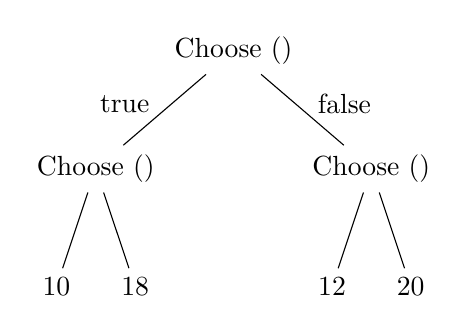
\begin{tikzpicture}[level distance=1.5cm,
level 1/.style={sibling distance=3.5cm},
level 2/.style={sibling distance=1cm}]
%\tikzstyle{every node}=[circle,draw]

\node (Root) [draw=none,rectangle] {Choose ()}
    child { node[draw=none] (q0) {Choose ()} 
      child { node[draw=none] (q00) {10}
      }
      child { node[draw=none] (q01) {18} 
      }
      edge from parent node [draw=none,left,xshift=-2.0,yshift=2.0] {true}
    }
    child { node [draw=none] (q1) {Choose ()}
      child { node[draw=none] (q10) {12}
      }
      child { node[draw=none] (q11) {20}       
      }
      edge from parent node [draw=none,right,xshift=2.0,yshift=2.0] {false}
    };
\end{tikzpicture}
\end{center}\caption{Interpretation of the conditional expression as a computation tree. The left edges correspond to \code{Choose} being instantiated with \code{true}. Analogously, the right edges correspond to an instantiation of \code{Choose} with \code{false}.}\label{fig:condexp}
\end{figure}

During evaluation of the expression we eventually have to interpret the root node \type{Choose} in Figure \ref{fig:condexp} and possibly its immediate subtrees.
There are multiple possible interpretations. One interpretation is to always interpret \type{Choose} as \code{true} which figuratively corresponds to taking the left branch. The node we arrive at is also a \type{Choose}-node, so again we choose the left branch to arrive at a leaf that contains the concrete value $10$. Hence under this interpretation the handler collapses the computation tree into the leaf $10$. Dually, we could always choose false which leads to the output value $20$. Figures \ref{fig:positive} and \ref{fig:negative} illustrate the two interpretations respectively.
\begin{figure}[b!]
    \centering
    \begin{subfigure}[t]{0.5\textwidth}
        \centering
\begin{tikzpicture}[level distance=1.5cm,
level 1/.style={sibling distance=3.5cm},
level 2/.style={sibling distance=1cm}]
%\tikzstyle{every node}=[circle,draw]

\node (Root) [draw=none,rectangle] {Choose ()}
    child { node[draw=none] (q0) {Choose ()} 
      child { node[draw=none] (q00) {10}
      }
      child { node[draw=none] (q01) {18} 
      }
      edge from parent node [draw=none,left,xshift=-2.0,yshift=2.0] {true}
    }
    child { node [draw=none] (q1) {Choose ()}
      child { node[draw=none] (q10) {12}
      }
      child { node[draw=none] (q11) {20}       
      }
      edge from parent node [draw=none,right,xshift=2.0,yshift=2.0] {false}
    };
\draw[->,black,rounded corners,dashed,line width=0.7pt]
     ($(Root) +(-1.0,0.2)$) --
     ($(q0) +(-1.0,0.4)$) --
     ($(q00) +(-0.3,0.0)$);
\end{tikzpicture}
        \caption{The ``positive'' interpretation: Always choose true. Output: 10.}\label{fig:positive}
    \end{subfigure}%
    ~ 
    \begin{subfigure}[t]{0.5\linewidth}
        \centering
 \begin{tikzpicture}[level distance=1.5cm,
level 1/.style={sibling distance=3.5cm},
level 2/.style={sibling distance=1cm}]
%\tikzstyle{every node}=[circle,draw]

\node (Root) [draw=none,rectangle] {Choose ()}
    child { node[draw=none] (q0) {Choose ()} 
      child { node[draw=none] (q00) {10}
      }
      child { node[draw=none] (q01) {18} 
      }
      edge from parent node [draw=none,left,xshift=-2.0,yshift=2.0] {true}
    }
    child { node [draw=none] (q1) {Choose ()}
      child { node[draw=none] (q10) {12}
      }
      child { node[draw=none] (q11) {20}       
      }
      edge from parent node [draw=none,right,xshift=2.0,yshift=2.0] {false}
    };
\draw[->,black,rounded corners,dashed,line width=0.7pt]
     ($(Root) +(1.0,0.2)$) --
     ($(q1) +(1.0,0.4)$) --
     ($(q10) +(1.3,0.0)$);
\end{tikzpicture}
        \caption{The ``negative'' interpretation: Always choose false. Output: 20.}\label{fig:negative}
    \end{subfigure}\caption{Two different interpretations.}    
\end{figure}
Alternatively, we could make a random choice between true and false at each branch. Again, this interpretation leads to one single output value. Albeit, the output value would be non-deterministic under this interpretation. 

Yet another interpretation is to enumerate all possible choices. For example, we can decide to explore the left branch and thereafter the right branch at each node. This interpretation corresponds to performing a depth-first traversal of the computation tree. Therefore, under this interpretation the computation tree collapses into a set of its leaves. Figure \ref{fig:enumerate} illustrates the tree traversal.
\begin{figure}[t]
\begin{center}
\begin{tikzpicture}[level distance=1.5cm,
level 1/.style={sibling distance=3.5cm},
level 2/.style={sibling distance=1cm}]
%\tikzstyle{every node}=[circle,draw]
\node (Root) [draw=none,rectangle] {Choose ()}
    child { node[draw=none] (q0) {Choose ()} 
      child { node[draw=none] (q00) {10}
      }
      child { node[draw=none] (q01) {18} 
      }
      edge from parent node [draw=none,left,xshift=-2.0,yshift=2.0] {true}
    }
    child { node [draw=none] (q1) {Choose ()}
      child { node[draw=none] (q10) {12}
      }
      child { node[draw=none] (q11) {20}       
      }
      edge from parent node [draw=none,right,xshift=2.0,yshift=2.0] {false}
    };
\draw[->,black,rounded corners,dashed,line width=0.7pt]
     ($(Root) +(-1.0,0.2)$) --
     ($(q0) +(-1.0,0.4)$) --
     ($(q00)  +(-0.5,0.0)$) --
     ($(q00)  +(-0.4,-0.35)$) --
     ($(q00)  +(0.0,-0.5)$) --
     ($(q00)  +(0.4,-0.35)$) --
     ($(q00)  +(0.5,0.0)$) --
     ($(q0)  +(-0.005,-0.3)$) --
     ($(q01)  +(-0.35,-0.35)$) --
     ($(q01)  +(0.0,-0.45)$) --
     ($(q01)  +(0.35,-0.35)$) --
     ($(q01)  +(0.4,0.0)$) --
     ($(q0)   +(1.0,0.5)$) --
     ($(Root) +(-0.3,-0.4)$) --
     ($(q1)  +(-0.8,-0.1)$) --
     ($(q10)  +(-0.5,0.0)$) --
     ($(q10)  +(-0.4,-0.35)$) --
     ($(q10)  +(0.0,-0.5)$) --
     ($(q10)  +(0.4,-0.35)$) --
     ($(q10)  +(0.5,0.0)$) --
     ($(q1)  +(-0.005,-0.3)$) --
     ($(q11)  +(-0.35,-0.35)$) --
     ($(q11)  +(0.0,-0.45)$) --
     ($(q11)  +(0.35,-0.35)$) --
     ($(q11)  +(0.4,0.0)$);
\end{tikzpicture}\caption{Enumerate all possible choices. Output: $\{10,18,12,20\}$.}\label{fig:enumerate}
\end{center}
\end{figure}

Essentially, our interpretations (handlers) correspond to particular folds over syntax trees (abstract computations) \cite{Kammar2013}.
\section{Row polymorphism}\label{sec:rowpolymorphism}
Row polymorphism is a typing discipline for records \cite{Remy1993}. A record is an unordered collection of fields, e.g. $\record{l_1 : t_1,\dots,l_n : t_n}$ denotes a record type with $n$ fields where $l_i$ and $t_i$ denote the name and type, respectively, of the $i$th field. Moreover, the record type is monomorphic, that is, the type is fixed. Row polymorphism, as the name suggests, makes record types polymorphic.

The following illustrates the power of row polymorphism.
\begin{example}
OCaml's (regular) record types are monomorphic.\footnote{OCaml's object types are row polymorphic.} Consider the following two record type definitions in OCaml
\begin{lstlisting}[style=ocaml]
type student    = {name : string; id : string}
type supervisor = {name : string; group : string} 
\end{lstlisting}
Now we can create instances of \type{student} and \type{supervisor}
\begin{lstlisting}[style=ocaml]
ocaml> let daniel = {name="Daniel"; id="s1467124"};;
val daniel : person = {name="Daniel"; id="s1467124"}

ocaml> let sam = {name="Sam"; group="LFCS"};;
val sam : supervisor = {name="Sam"; group="LFCS"}
\end{lstlisting}
As expected the OCaml compiler infers the correct record types for both instances. Since both record types have the field \emph{name} in common we might expect to define a function which prints the name field of either record type, e.g.
\begin{lstlisting}[style=ocaml]
ocaml> let print_name r = r.name;;
ocaml> let () = 
         print_name daniel;
         print_name sam;;
\end{lstlisting}
Surprisingly this yields the following type error
\begin{lstlisting}[style=ocaml]
         print_name daniel;
                    ^^^^^^
Error: This expression has type student
       but an expression was expected of type supervisor
\end{lstlisting}
The record \code{daniel} is not compatible with the type of \code{print\_name}. Because the record types are monomorphic, the compiler has to decide on compile time which record type \code{print\_name} accepts as input parameter. Apparently in this example the compiler has decided to type \code{print\_name} as \type{supervisor $\to$ string}.

Now consider the same example in Links. In contrast to OCaml record types are polymorphic in Links.
First we define the \code{print\_name} function
\begin{lstlisting}[style=links]
links> fun print_name(r) { r.name };
print_name = fun : ((name:a|§*$\rho$*§)) ~> a
\end{lstlisting}
Links tells us that the function accepts a record type which has \emph{at least} the field \type{name}. The field type is polymorphic as signified by the presence of the type variable \type{a}. The additional type variable $\rho$ is a polymorphic row variable which can be instantiated to additional fields, hence the actual input record may contain \emph{more} fields. Now our printing function works as expected:
\begin{lstlisting}[style=links]
links> fun(){ print_name(daniel);
              print_name(sam) }();
Daniel
Sam
\end{lstlisting}
Here we wrapped the applications of \code{print\_name} inside a parameterless function because Links does not support expression sequencing in the top-level.
\end{example}
More on $\rho$, unification, etc\dots
% Records are unordered collections of fields, e.g. $\record{l_1:t_1,\dots,l_n : t_n}$ denotes a record type with $n$ fields where $l_i$ and $t_i$ denote the name and type, respectively, of the $i$th field.
% Records are particularly great for structuring related data.
% For example the record instance $\record{name="Daniel", age=25}$ could act as simple description of a person.
% A possible type for the record would be $\record{name : \typename{string}, age : \typename{int}}$.
% The implicit ordering of fields in records is not important as the following two types are considered equivalent:
% \[ \record{name : \typename{string}, age : \typename{int}} \equiv \record{age : \typename{int}, name : \typename{string}}. \]
% The equivalence captures what is meant by \emph{unordered} collection of fields.

% We can define functions that work on records, for example, occasionally we might find it useful to retrieve the name field in an instance of the person-record:
% \[ \text{name}_1 = \lambda x . (x.name). \]
% We can apply $\text{name}_1$ to the above record instance, e.g. 
% \[ \text{name}_1(\record{name="Daniel", age=25}) = "Daniel" \] 
% yields the expected value.
% The question remains which type the function $\text{name}_1$ has.
% For this particular example the type $\record{name : \typename{string}} \to \typename{string}$ seems reasonable.

% Now, consider the following function takes a record and returns a pair where the first component contains the value of the name field and the second component contains the input record itself:
% \[ \text{name}_2 = \lambda x . (x.name, x) \]
% Again, we ask ourselves what is the type of $\text{name}_2$?
% The function must have type $\record{name : \typename{string}} \to \typename{string} \times \record{name : \typename{string}}$.
% This type appears innocuous, but consider the consequence of
% \[ \text{let }(n, r) = \text{name}_2(\record{name="Daniel", age=25}). \]
% Now, $n$ has type $\typename{string}$ as desired, but $r$ has type \record{name : \typename{string}}.
% In other words, we have lost the field ``age''.
% This example is a particular instance of the \emph{loss of information} problem.

% Row polymorphism was conceived to address this problem. 
% Row polymorphism is powerful a typing discipline for typing records \cite{Remy1993}.
% The principal idea is to extend record types with a \emph{polymorphic row variable}, $\rho$, which can be instantiated with additional fields.
% For example with row polymorphism our function $\text{name}_2$ would have type $\record{name : \typename{string} \; | \; \rho }$, and $r$ in the previous example would be assigned the type $\record{name : \typename{string}, age : \typename{int} \; | \; \rho }$.
% Now, we have no longer lose information.

% \subsection{Type theoretic row polymorphism}
% \subsection{Row polymorphism is not subtyping}
% Programming with handlers chapter
\chapter{Programming with handlers in Links}\label{ch:programming}
Through a series of examples we will explore programming with two types of effect handlers in Links. Section \ref{sec:closedhandlers} introduces \emph{closed handlers} and in particular emphasises the high degree of modularity afforded by closed handlers. Section \ref{sec:openhandlers} introduces the slightly more generalised \emph{open handlers} and focuses mainly on the compositionality of (open) handlers.

\section{Discharging operations in Links}\label{sec:discharge}
Syntactically an operation is similar to variant types in Links. Every operation name starts with a capital letter, e.g. \type{Get}, \type{Put}, etc. Every operation takes an input and yields an output. The output from discharging an operation is entirely decided by effect handlers in the evaluation context. That is, alone an operation does not have any semantics.

Operations are discharged using the \code{do}-primitive. However discharging an operation in an unhandled context yields an evaluation error:
\begin{lstlisting}[style=links]
links> do Get();
*** Error: Unhandled operation: Get()
\end{lstlisting}
The typing of operations is uniform because every operation takes exactly one input. Therefore the type of an operation is on the form $a \to b$ where $a$ and $b$ are type variables. In order to simulate multiple parameters one can instantiate $a$ to a record type, e.g. $\code{Put}((\code{true},1))$ is an operation of type $(\type{Bool},\type{Int}) \to b$.

Similarly, one can simulate a nullary operation by passing the empty record, e.g. $\code{Get}()$ has type $() \to b$.

\section{Closed handlers}\label{sec:closedhandlers}
A closed handler handles a fixed set of effects, that is, it effectively describes an upper bound on which kind of effects a computation may perform. In Links this bound is made explicit in the handler's type, e.g. the closed handler \code{h}
\begin{lstlisting}[style=links]
var h = handler(m) {
  case Op(p,_)   -> p
  case Return(x) -> x
}
\end{lstlisting}
has the type $\chntype{\thunktype{Op : a \to a}{a}}{a}$ where the absence of a row variable in the effect signature implies that the computation \code{m} may not perform any other effects than \type{Op}. It is considered a type error to handle a computation whose effect signature is larger than the handler supports. 

This restriction introduces slack into the type system. To illustrate the slack consider the following computation
\begin{lstlisting}[style=links]
fun comp() {
  do Op(true);
  if (false == true) {
    do Op2(false)
  } else { 
    true
  }
}
\end{lstlisting}
The computation \code{comp} has type $\thunktype{Op:\type{Bool} \to (),Op2:\type{Bool} \to \type{Bool} \; | \; \rho}{\type{Bool}}$. Obviously, \code{Op2} never gets discharged. However, attempting to handle \code{comp} with the handler \code{h} yields a type error because \code{Op2} is present in the effect signature of \code{comp}. The type system is conservative, but in general it is undecidable whether the first or second branch of a conditional expression will be taken \cite{Huttel2010}.

The following sections will show increasingly interesting examples of programming with closed handlers in Links.

\subsection{Transforming the results of computations}\label{sec:transform}
Handlers take computations as input. From a handler's perspective a computation is a \emph{thunk}, i.e. a parameterless function whose type is similar to $\thunktype{Op_i:a_i \to b_i}{c}$. The first few examples show how to transform the output of a computation using handlers. We begin with a handler that appears to be rather boring, but in fact proves very useful as we shall see later in Section \ref{sec:openhandlers}.
\begin{example}[The force handler]\label{ex:force}
We dub the handler \code{force} as it takes a computation (thunk) as input, evaluates it and returns its result. It has type $\code{force} : (() \to a) \to a$ and it is defined as
\begin{lstlisting}[style=links]
var force = handler(m) {
    case Return(x) -> x
}
\end{lstlisting}
Essentially, this handler applies the identity transformation to the result of the computation \code{m}. Running \code{force} on a few examples should yield no surprises:
\begin{lstlisting}[style=links]
fun fortytwo() { 42 }
links> force(fortytwo);
42 : Int

fun hello() { "Hello" }
links> force(hello);
"Hello" : String
\end{lstlisting}
The handler \code{force} behaves as expected for these trivial examples. But suppose we want to print ``\emph{Hello World}'' to the standard output, e.g.
\begin{lstlisting}
fun print_hello() { print("Hello World") }
links> force(print_hello);
Type error: §*\dots*§ # Omitted for brevity
\end{lstlisting}
then the Links compiler contemptuously halts with a type error! The type of \code{print\_hello} is $() \rightsquigarrow ()$ which at first glance may appear to be compatible with the type of formal parameter \code{m}. But printing to standard output is effectful action, as indicated by the squiggly arrow in the signature, hence \code{print\_hello} is an effectful computation. Since \code{force} does not handle any effects we get the type error. 
\end{example}
As Example \ref{ex:force} demonstrated the handler \code{force} could not handle the print effect caused by \code{print\_hello}. In fact no handler in Links is able to handle \code{print\_hello} because the print effect is a syntactic, built-in effect known as \emph{wild}. Handlers only handles user-defined effects.

The next example demonstrates an actual transformation.
\begin{example}[The listify handler]\label{ex:listify}
The \code{listify} handler transforms the result of a handled computation into a singleton list. Its type is $\code{listify} : (() \to a) \to [a]$ and its definition is straightforward
\begin{lstlisting}[style=links]
var listify = handler(m) {
  case Return(x) -> [x]
}
\end{lstlisting}
When handling the computations from Example \ref{ex:force} we see that it behaves as expected, e.g.
\begin{lstlisting}[style=links]
links> listify(fortytwo);
[42] : [Int]

links> listify(hello);
["Hello"] : [String]

fun list123() { [1,2,3] }
links> listify(list123);
[[1,2,3]] : [[Int]]
\end{lstlisting}
These examples also illustrate the \code{Return}-case serves a similar purpose to the monadic \code{return}-function in Haskell whose type is $\code{return} : a \to m\, a$ for a monad $m$. It ``lifts'' the result into an adequate type.
\end{example}

In a similar fashion to the handler \code{listify} in Example \ref{ex:listify} we can define handlers that increment results by 1, perform a complex calculation using the result of the computation or wholly ignore the result. The bottom line is that it must ensure its output has an adequate type. In the case for \code{listify} the type must be a list of whatever type the computation yielded.

\subsection{Exception handling}\label{sec:maybehandler}
Until now we have only seen some simple transformations. Let us spice things up a bit. 
Example \ref{ex:maybe} introduces the practical handler \code{maybe}. It is similar to the \type{Maybe}-monad in Haskell. For reference we briefly sketched the behaviour of the \type{Maybe}-monad in Section \ref{sec:problem-with-monads}.
\begin{example}[The maybe handler]\label{ex:maybe}
The \type{maybe} handler handles one operation $\type{Fail} : a \to a$ that can be used to indicate that something unexpected has happened in a computation. The handler returns \type{Nothing} when \type{Fail} is raised, and \type{Just} the result when the computation succeeds, thus its type is
\[ \code{maybe} : \chntype{\thunktype{\type{Fail} : a \to a}{b}}{[|\type{Just}:b|\type{Nothing}|\rho|]}. \]
It is defined as
\begin{lstlisting}[style=links]
var maybe = handler(m) {
  case Fail(_,_) -> Nothing
  case Return(x) -> Just(x)
}
\end{lstlisting}
When a computation raises \type{Fail} the handler discards the remainder of the computation and returns \type{Nothing} immediately, e.g.
\begin{lstlisting}[style=links]
fun yikes() { 
  var x = "Yikes!";
  do Fail();
  x
}
links> maybe(yikes);
Nothing() : [|Just:String|Nothing|§*$\rho$*§|]
\end{lstlisting}
and if the computation succeeds it transforms the result, e.g.
\begin{lstlisting}[style=links]
fun success() {
  true
}
links> maybe(success);
Just(true) : [|Just:Bool|Nothing|§*$\rho$*§|]
\end{lstlisting}
\end{example}
The next example demonstrates an alternative ``exception handling strategy''.
\begin{example}[The recover handler]\label{ex:recover}
We can define a handler \code{recover} which ignores the raised exception and resumes execution of the computation.
The type of \code{recover} is
\[ \code{recover} : \chntype{\thunktype{\type{Fail}: a \to ()}{b}}{[|\type{Just}:b|\rho|]}. \]
A slight reminder here: The label \type{Nothing} is absent from the handler's output type because \type{Just} is a polymorphic variant label and its relation to \type{Nothing} is conventional. We define \code{recover} as
\begin{lstlisting}[style=links]
var recover = handler(m) {
  case Fail(_,k) -> k(())
  case Return(x) -> Just(x)
}
\end{lstlisting}
In contrast to \code{maybe} from Example \ref{ex:maybe} the \code{recover} handler invokes the continuation \code{k} once. This invocation effectively resumes execution of the computation. Consider \code{recover} applied to the computation \code{yikes} from before
\begin{lstlisting}[style=links]
links> recover(yikes)
Just("Yikes!") : [|Just:String|§*$\rho$*§|]
\end{lstlisting}
\end{example}
Although it is seldom a sound strategy to ignore exceptions the two Examples \ref{ex:maybe} and \ref{ex:recover} demonstrate that we can change the semantics of the computation by changing the handler.
\section{Open handlers}

\subsection{An effectful coffee dispenser in Links}
In Section \ref{sec:monads} we implemented a basic coffee dispenser model in Haskell using monads (Example \ref{ex:coffee1}). However, it was difficult to extend the model to include more properties like writing to a display and system failures due to monads' lack of compositionality.

In contrast (open) handlers enable us implement a modular coffee dispenser model in Links. Example \ref{ex:coffee-links} implements the model and Example \ref{ex:coffee-links2} demonstrates how the modularity and compositionality of handlers lets us change the behaviour of the coffee dispenser without breaking a sweat.
\begin{example}[Coffee dispenser]\label{ex:coffee-links}
The coffee dispenser performs two operations directly
\begin{enumerate}
  \item \type{Ask}: Retrieves the inventory.
  \item \type{Tell}: Writes a description of the item to some medium.
\end{enumerate}
Indirectly, the coffee dispenser may perform the \type{Fail} operation when it looks up an item. Thus the type of the dispenser is 
\[ \code{dispenser} : a \xrightarrow{\{\type{Ask}:() \to [(a, b)], \type{Fail}:() \to b,\type{Tell}:b \to c| \rho\}\;} c \]
We compose the coffee dispenser from the aforementioned operations and the look-up function, e.g.
\begin{lstlisting}[style=links]
fun dispenser(n) {
  var inv = do Ask();
  var item = lookup(n,inv);
  do Tell(item)
}
\end{lstlisting}
The monadic coffee dispenser model used three monads: \type{Reader}, \type{Writer} and \type{Maybe} to model the desired behaviour. We will implement three handlers which resemble the monads. First, let us implement \type{Reader}-monad as the handler \code{reader} whose type is 
\[  (() \xrightarrow{\{\type{Ask}:(a) \to [(\type{Int}, [|\type{Coffee}|\type{Tea}|\rho_1|])] \, | \,\rho_2\}\;} b) -> () \xrightarrow{\{\type{Ask}:\alpha|\rho_2\}\;} b \]
For simplicity we hard-code the inventory into the handler
\begin{lstlisting}[style=links]
open handler reader(m) {
  case Ask(_,k)  -> k([(1,Coffee),(2,Tea)])
  case Return(x) -> x
}
\end{lstlisting}
When handling the operation \type{Ask} the handler simply invokes the continuation \code{k} with the inventory as parameter. Like in Example \ref{ex:coffee1} we model the inventory as an association list.

Second, we implement the handler \code{writer} which provide capabilities to write to a medium. We let the medium be a regular string. The handler's type is
\[  (() \xrightarrow{\{\type{Tell}: [|\type{Coffee}|\type{Tea}|] \to \type{String} \, | \,\rho\}\;} a) -> () \xrightarrow{\{\type{Tell}:\alpha|\rho_2\}\;} a \]
and its definition is
\begin{lstlisting}[style=links]
open handler writer(m) {
  case Tell(Coffee,k) -> k("Coffee")
  case Tell(Tea,k)    -> k("Tea")
  case Return(x)      -> x
}
\end{lstlisting}
Here we use pattern-matching to convert \type{Coffee} and \type{Tea} into their respective string representations.

Finally, we implement the \code{lookup} function which given a key and an association list returns the element associated with the key if the key exists in the list, otherwise it discharges the \type{Fail}-operation to signal failure
\begin{lstlisting}[style=links]
fun lookup(n, xs) {
  switch (xs) {
    case [] -> do Fail()
    case ((i, e) :: xs) -> if (n == i) { e }
                          else { lookup(n, xs) }
  }
}
\end{lstlisting}
To handle failure we reuse the \type{maybe}-handler from Section \ref{sec:maybehandler} with the slight change that we make it an open handler. Now, we just have to glue all the components together
\begin{lstlisting}[style=links]
fun runDispenser(n) {
  force(maybe(writer(reader(fun() { dispenser(n) }))))
}
\end{lstlisting}
Note, that in this example the order in which we compose handlers is irrelevant.
Running a few examples we see that it behaves similarly to the monadic version we implemented in Section \ref{sec:monadtransformers}
\begin{lstlisting}[style=links]
links> runDispenser(1)
Just("Coffee") : [|Just:String|Nothing|§*$\rho$*§|]

links> runDispenser(2)
Just("Tea") : [|Just:String|Nothing|§*$\rho$*§|]

links> runDispenser(3)
Nothing() : [|Just:String|Nothing|§*$\rho$*§|]
\end{lstlisting}
\end{example}

\subsection{Reinterpreting Nim}
% Implementation
\chapter{Implementation}
The Links compiler is a multi-pass compiler with several distinct phases.
Coarsely, we can divide the compiler into two major components the front-end and back-end.
We can further subdivide the front-end into
\begin{itemize}
  \item Parser: Transforms the input source into a syntax tree.
  \item Early desugar: Performs source-to-source transformations before source analysis.
  \item Type checker: Analyses the source, performs type inference, and ensures terms are well-typed.
\end{itemize}
The compiler has more front-end components, but these are the most relevant for our implementation.
Similarly, the back-end can be further subdivided
\begin{itemize}
  \item IR Compiler: Transforms the source into an intermediate representation used by the interpreter.
  \item Pattern-matching compiler: Aids the IR compiler by compiling pattern-matching constructs into the intermediate representation.
\end{itemize}
Figure \ref{fig:compiler-phases} provides a high level picture of how the different relevant phases are connected. The subsequent sections discuss implementation specific details.
\begin{figure}[t]
\begin{center}
\tikzset{my ellipse/.style={
        draw=blue, 
        ultra thick, 
        rectangle, 
        anchor=west, 
        xshift=1.0cm},
}
\tikzset{my rectangle/.style={
        draw=black, 
        thick, 
        rectangle, 
        minimum width={width("Early desugar")+2pt}}
}
\tikzset{my arrow/.style={-latex, thick}}

\begin{tikzpicture}  
  % Frontend
  \node [my rectangle,draw=black,thick] (Early desugar) at (0,0) {Early desugar};
  \node [my rectangle,draw=black,thick,above of=Early desugar] (Parser) {Parser};
  \node [my rectangle,draw=black,thick,below of=Early desugar] (Typechecker) {Type checker};
  %\node [my rectangle,draw=black,thick,below of=Typechecker] (Late desugar) {Late desugar};

  \node[rectangle,draw=black,ultra thick,minimum height=+5.0cm,minimum width=+4.0cm,fit ={(Parser.north) (Typechecker.south)}] (Frontend) {};

  % Input source
  \node [rectangle,draw=black,thick,xshift=-3.0cm,left of=Frontend] (Source) {Source};

  % Backend
  \node [my rectangle,xshift=+4.0cm,draw=black,thick,right of=Parser] (Sugartoir) {IR Compiler};
  \node [my rectangle,yshift=-0.5cm,draw=black,thick,below of=Sugartoir] (PMC) {\begin{tabular}{l}Pattern\\Matching\\ Compiler\end{tabular}};
  
  \node[rectangle,draw=black,ultra thick,minimum width=+4.0cm,minimum height=+5.0cm,fit ={(Sugartoir.north) (PMC.south)}] (Backend) {};

  % Interpreter
  \node [rectangle,xshift=+3.5cm,draw=black,thick,right of=Backend] (Evalir) {Interpreter};

  % Texts
  \node [anchor=north, font=\bfseries,yshift=-0.1cm] at (Frontend.north) {Frontend};
  \node [anchor=north, font=\bfseries,yshift=-0.1cm] at (Backend.north) {Backend};

  % Arrows
  \draw [->, ultra thick] (Source.east) -- (Frontend.west) {};
  \draw [->, ultra thick] (Frontend.east) -- (Backend.west) {};
  \draw [->, ultra thick] (Backend.east) -- (Evalir.west) {};

  \draw [->, thick] (Parser.south) -- (Early desugar.north) {};
  \draw [->, thick] (Early desugar.south) -- (Typechecker.north) {};

  \draw [->, thick,out=150, in=20] (Sugartoir.-10.-150) -- (PMC.135.0) {};
  \draw [->, thick] (PMC.43.0) -- (Sugartoir.-19.0) {};
\end{tikzpicture}
\caption{Links compiler phases overview.}\label{fig:compiler-phases}
\end{center}
\end{figure}

\section{Early desugaring of handlers}
The \code{handler} and \code{open handler} constructs are syntactic sugar. They get desugared into a legacy construct from an early implementation. The initial implementation used a \code{handle}-construct for handlers. Figure \ref{fig:closedhandler-desugar} displays the conceptual transformation of \code{handler} to \code{handle}. 
This desugaring takes place right after the parsing phase. The early desugaring is beneficial because it allows us to take full advantage of the earlier implementation, whilst providing a more convenient syntax for handlers.
\begin{figure}[h]
    \centering
    \begin{subfigure}[c]{0.45\textwidth}
        \centering
\begin{lstlisting}[style=links]
handler(m) {
  case Op§*$_i$*§(p§*$_i$*§,k§*$_i$*§) -> b§*$_i$*§
  case Return(x) -> b
}
\end{lstlisting}
    \end{subfigure}%
    ~ 
    \begin{subfigure}[c]{0.1\textwidth}
      $\Rightarrow$
    \end{subfigure}%
    ~
    \begin{subfigure}[c]{0.45\textwidth}
        \centering
\begin{lstlisting}[style=links]
fun(m) {
  handle(m) {
    case Op§*$_i$*§(p§*$_i$*§,k§*$_i$*§) -> b§*$_i$*§
    case Return(x) -> b
  }
}
\end{lstlisting}
    \end{subfigure}
\caption{The \code{handler}-construct gets desugared into a \code{handle}-construct where the computation $m$ is abstracted over using a function.}\label{fig:closedhandler-desugar}
\end{figure}

The \code{open handler}-constructs get desugared in a similar fashion, but, with a small twist: The \code{handle}-construct gets wrapped inside a thunk. The extra layer of indirection entailed by this transformation is \emph{the key} to make handlers composable. The crucial insight is that by transforming every open handler into a thunk compositionality follows for free because computations are modelled as thunks.
Figure \ref{fig:openhandler-desugar} shows the conceptual transformation for \code{open handler}-constructs.

\begin{figure}[h]
    \centering
    \begin{subfigure}[c]{0.45\textwidth}
        \centering
\begin{lstlisting}[style=links]
open handler(m) {
  case Op§*$_i$*§(p§*$_i$*§,k§*$_i$*§) -> b§*$_i$*§
  case Return(x) -> b
}
\end{lstlisting}        
    \end{subfigure}%
    ~ 
    \begin{subfigure}[c]{0.1\textwidth}
      $\Rightarrow$
    \end{subfigure}%
    ~
    \begin{subfigure}[c]{0.45\textwidth}
        \centering
\begin{lstlisting}[style=links]
fun(m) {
  fun() {
    handle(m) {
      case Op§*$_i$*§(p§*$_i$*§,k§*$_i$*§) -> b§*$_i$*§
      case Return(x) -> b
    }
  }
}
\end{lstlisting}       
    \end{subfigure}
\caption{The \code{open handler}-construct gets desugared into a thunked \code{handle}-construct.}\label{fig:openhandler-desugar}
\end{figure}

\section{Type inference}
\section{Pattern-matching compilation}
Syntactically, the \code{handler}-construct and \code{switch}-construct are similar. Figure \ref{fig:handler-switch} puts the two construct side-by-side.
\begin{figure}[h]
    \centering
    \begin{subfigure}[c]{0.45\textwidth}
        \centering
\begin{lstlisting}[style=links]
handler(m) {
  case Op§*$_i$*§(p§*$_i$*§,k§*$_i$*§) -> b§*$_i$*§
  case Return(x) -> b
}
\end{lstlisting}        
    \end{subfigure}%  
    ~
    \begin{subfigure}[c]{0.45\textwidth}
        \centering
\begin{lstlisting}[style=links]
switch(x) {
  case §*$\textit{Pattern}_j$*§ -> b§*$_j$*§
  case other   -> b§*$'$*§
}
\end{lstlisting}       
    \end{subfigure}
\caption{The \code{handler}-construct resembles the \code{switch}-construct syntactically.}\label{fig:handler-switch}
\end{figure}
Notably, their semantics differ as \code{switch} allows arbitrary pattern matching on an expression $x$ and \code{handler} only allows pattern matching on possible operation names in some computation $m$. Furthermore, \code{switch} has a default case \code{other} which is not allowed in \code{handler}. The resemblance has certain benefits:
\begin{itemize}
  \item Syntactical commonalities makes handlers feel like a natural integrated part in Links,
  \item and we can reuse the \code{switch} infrastructure for \code{handler}.
\end{itemize}

\section{Interpreter}
The intermediate representation used by the Links compiler is a variant of A-normalform (ANF) \cite{Flanagan1993}. In particular, the Links interpreter directly interprets the ANF code \cite{Lindley2012}.

\section{Early desugaring of handlers}
The \code{handler} and \code{open handler} constructs are syntactic sugar. They get desugared into a legacy construct from an early implementation. The initial implementation used a \code{handle}-construct for handlers. Figure \ref{fig:closedhandler-desugar} displays the conceptual transformation of \code{handler} to \code{handle}. 
This desugaring takes place right after the parsing phase. The early desugaring is beneficial because it allows us to take full advantage of the earlier implementation, whilst providing a more convenient syntax for handlers.
\begin{figure}[h]
    \centering
    \begin{subfigure}[c]{0.45\textwidth}
        \centering
\begin{lstlisting}[style=links]
handler(m) {
  case Op§*$_i$*§(p§*$_i$*§,k§*$_i$*§) -> b§*$_i$*§
  case Return(x) -> b
}
\end{lstlisting}
    \end{subfigure}%
    ~ 
    \begin{subfigure}[c]{0.1\textwidth}
      $\Rightarrow$
    \end{subfigure}%
    ~
    \begin{subfigure}[c]{0.45\textwidth}
        \centering
\begin{lstlisting}[style=links]
fun(m) {
  handle(m) {
    case Op§*$_i$*§(p§*$_i$*§,k§*$_i$*§) -> b§*$_i$*§
    case Return(x) -> b
  }
}
\end{lstlisting}
    \end{subfigure}
\caption{The \code{handler}-construct gets desugared into a \code{handle}-construct where the computation $m$ is abstracted over using a function.}\label{fig:closedhandler-desugar}
\end{figure}

The \code{open handler}-constructs get desugared in a similar fashion, but, with a small twist: The \code{handle}-construct gets wrapped inside a thunk. The extra layer of indirection entailed by this transformation is \emph{the key} to make handlers composable. The crucial insight is that by transforming every open handler into a thunk compositionality follows for free because computations are modelled as thunks.
Figure \ref{fig:openhandler-desugar} shows the conceptual transformation for \code{open handler}-constructs.

\begin{figure}[h]
    \centering
    \begin{subfigure}[c]{0.45\textwidth}
        \centering
\begin{lstlisting}[style=links]
open handler(m) {
  case Op§*$_i$*§(p§*$_i$*§,k§*$_i$*§) -> b§*$_i$*§
  case Return(x) -> b
}
\end{lstlisting}        
    \end{subfigure}%
    ~ 
    \begin{subfigure}[c]{0.1\textwidth}
      $\Rightarrow$
    \end{subfigure}%
    ~
    \begin{subfigure}[c]{0.45\textwidth}
        \centering
\begin{lstlisting}[style=links]
fun(m) {
  fun() {
    handle(m) {
      case Op§*$_i$*§(p§*$_i$*§,k§*$_i$*§) -> b§*$_i$*§
      case Return(x) -> b
    }
  }
}
\end{lstlisting}       
    \end{subfigure}
\caption{The \code{open handler}-construct gets desugared into a thunked \code{handle}-construct.}\label{fig:openhandler-desugar}
\end{figure}
\section{Type checking}
The type checker implements the following typing rule for open handlers \cite{Kammar2013}:
\begin{equation}\label{eq:typing}
\mprset{flushleft}
\inferrule{E_{in} \defas \{\type{Op}_i : A_i \to B_i\}_i \uplus \rho \\\\
           E_{out} \defas E_{forward} \uplus \rho\\\\
           H \defas \{\code{Return}(x) \mapsto M\} \uplus \{\type{Op}_i(p,k) \mapsto N_i\}_i \\\\
          \left( \varGamma, p : A_i, k : U_{E_{out}}(B_i \to C) \vdash_{E_{out}} N_i : C \right)_i \\\\
          \varGamma, x : A \vdash_{E_{out}} M : C}
          {\varGamma \vdash H : A\, \overset{E_{in}\;\;\;E_{out}}{\Rightarrow} C}
\end{equation}
The typing rule for closed handlers is similar, however, it leaves out the row variable $\rho$.

\subsection{Implementation details}
The type checker for handlers take advantage of the existing infrastructure for the \code{switch}-construct which also embodies a collection of \code{case}-expressions. Figure \ref{fig:handler-switch} displays the two constructs side-by-side.

In order to determine which operations a handler handles the type checker invokes the type checking procedure for \code{case}-expressions. This procedure returns a list of the patterns being matched. In the concrete case for handlers the procedure infers that the \code{case}-expressions pattern match on a variant type. The tags in the variant are precisely the names of the operations that the handler handles. This also reveals why operations resemble variant constructors so closely.

Internally, a variant is represented by a row. So, the handler type checker extracts the row from the inferred variant type, thereafter it applies the typing rule \eqref{eq:typing} to turn obtain the desired effect row.
\section{Pattern-matching compilation}
Syntactically, the \code{handler}-construct and \code{switch}-construct are similar. Figure \ref{fig:handler-switch} depicts their similarities.
\begin{figure}[h]
    \centering
    \begin{subfigure}[c]{0.45\textwidth}
        \centering
\begin{lstlisting}[style=links]
handler(m) {
  case Op§*$_i$*§(p§*$_i$*§,k§*$_i$*§) -> b§*$_i$*§
  case Return(x) -> b
}
\end{lstlisting}        
    \end{subfigure}%  
    ~
    \begin{subfigure}[c]{0.45\textwidth}
        \centering
\begin{lstlisting}[style=links]
switch(e) {
  case §*$\textit{Pattern}_j$*§ -> b§*$_j$*§
  case other   -> b§*$'$*§
}
\end{lstlisting}       
    \end{subfigure}
\caption{The \code{handler}-construct resembles the \code{switch}-construct syntactically.}\label{fig:handler-switch}
\end{figure}
Notably, their semantics differ as \code{switch} allows arbitrary pattern matching on an expression $x$ and \code{handler} only allows pattern matching on possible operation names in some computation $m$. Furthermore, \code{switch} has a default case \code{other} which is not allowed in \code{handler}. 
Their syntactic similarities give rise to a similar internal representation as well. Although, the internal representation of \code{handler} contains extra attributes such as whether the handler is open or closed.
The resemblance has certain benefits:
\begin{itemize}
  \item Syntactical commonalities makes handlers feel like a natural integrated part in Links,
  \item and we can reuse the \code{switch} pattern-matching compilation infrastructure for \code{handler}.
\end{itemize}
The \code{switch} pattern-matching compiler supports deep pattern-matching which we want for matching on actual operation parameters, but only a handful of patterns are permitted for matching on continuation parameters. Figure \ref{fig:cont-pattern-matching} shows the legal pattern-matching on a continuation parameter. Moreover, the \code{Return}-case must only take one parameter. These small subtleties prevent us from using the \code{switch} pattern-matching compiler directly.

\begin{figure}[H]
\begin{center}
\begin{lstlisting}[style=links]
         handler(m) {
           case Op§*$_{i_1}$*§(_,k)      -> b§*$_{i_1}$*§  # Name binding
           case Op§*$_{i_2}$*§(_,k as c) -> b§*$_{i_2}$*§  # Aliasing
           case Op§*$_{i_3}$*§(_,_)      -> b§*$_{i_3}$*§  # Wildcarding
           case Return(x)     -> b§*$_{i_4}$*§
         }
\end{lstlisting}        
\end{center}
\caption{Permissible patterns for matching on the continuation parameter.}\label{fig:cont-pattern-matching}
\end{figure}

Instead we embed the \code{switch} pattern-matching compiler along with a preliminary pattern-matching analyser in the \code{handler} pattern-matching compiler. The pattern-matching analyser checks that the patterns are legal, i.e.
\begin{itemize}
  \item An operation-case has at least two parameters, where the last parameter is supposed to be the continuation.
  \item Pattern-matching on a continuation parameter is either name binding, aliasing or wildcarding.
  \item \code{Return}-case(s) only take one parameter.
\end{itemize}
If the pattern-matching analysis is successful then the \code{switch} pattern matching compiler is invoked to generate the code. Otherwise, a compilation error, complaining about illegal patterns, is emitted.
\section{Interpreter}
% Continuation passing style (CPS) is often used as an intermediate representation during the optimisation stage by functional compilers. In particular, CPS makes it easy to implement first-class control in the source level as CPS exposes the current continuation \cite{Appel2007}.

% A related intermediate representation is A-Normal Form (ANF) which is used by the Links compiler. Furthermore, the Links interpreter directly interprets ANF code \cite{Lindley2012}.
% ANF is a relatively simple language that enjoys many of the same advantages as CPS such as explicit exposure of the current continuation \cite{Flanagan1993}. However, CPS is better for performing optimisations, but the simpler nature of ANF makes it amendable as an interpreted language \cite{Appel2007,Flanagan1993}. 
The Links compiler uses A-Normal Form (ANF) as an intermediate representation. In particular, the Links interpreter directly interprets ANF code.
ANF is a relatively simple direct-style language which partitions expressions into two classes: atomic expressions and complex expressions. An expression is considered atomic if it is pure, i.e. it causes no effects and it terminates \cite{Flanagan1993}. On the other hand, every complex expression must be assigned a fresh name. For example the Links expression \code{g(f(h(x)))} gets translated into the Links-ANF computation \code{($\{$let y = h(x), let z = f(y)$\}$, g(z))} where the first component is a list of \code{let}-bound intermediate computations, and the second component is a tail computation. Incidentally, it is straightforward to implement first-class control in the source language as the current continuation can be built from the Links-ANF computation. Moreover, the simplicity of ANF makes it amendable as an interpreted language.

The Links interpreter is written in continuation-passing style (CPS) which threads the current continuation directly through the program. The continuation was implemented as a stack of continuation frames which capture computations along with their contexts. Formally, a continuation frame is quadruple $F \defas (\mathcal{S},\mathcal{B},\mathcal{E},\mathcal{C})$ where
\begin{itemize}
  \item $\mathcal{C}$ is a computation.
  \item $\mathcal{E}$ is an environment that binds names in $\mathcal{C}$.
  \item $\mathcal{B}$ is a binder for the computation.
  \item $\mathcal{S}$ denotes the scope of the computation.
\end{itemize}
For example the expression above gets encoded as the following continuation frame
\[ \left( \text{scope}(\code{y}), \code{y}, \text{localise}(\code{y}), \code{(\{let z = f(y)\}, g(z))} \right) \]
where scope and localise are two functions, that return the scope of a binder and localises the binder in the current environment, respectively.

This particular notion of continuation is problematic for handlers because we need delimited control for continuations assigned by handlers. Therefore it is necessary to generalise the notion of continuation in the Links interpreter. Fortunately, the generalisation is conceptual simple: Lift the continuation into a stack, i.e. let it become a stack of stacks of continuation frames. In other words the generalised continuation embeds the previous continuation layout. Figure \ref{fig:continuation-notion} illustrates the embedding. This scheme effectively turns every stack of continuation frames into a delimited continuation, i.e. a continuation that returns control to the caller.

\begin{figure}[H]
\begin{center}
\tikzset{my ellipse/.style={
        draw=blue, 
        ultra thick, 
        rectangle, 
        anchor=west, 
        xshift=1.0cm},
}
\tikzset{my rectangle/.style={
        draw=black, 
        thick, 
        rectangle, 
        minimum width={width("Early desugar")+2pt}}
}

\tikzset{my arrow/.style={-latex, thick}}

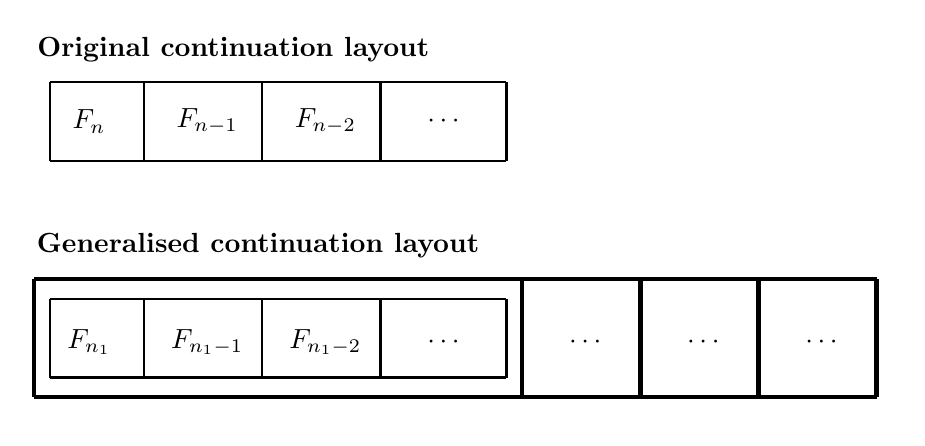
\begin{tikzpicture}  
  % Previous continuation
  % Draw rectangle
  \draw[thick,-] (-2.8,0) -- (-2.8,1.0) node[xshift=0.5cm] {};   % Left bar
  \draw[thick,-] (-2.8,1.0) -- (3.0,1.0) node[anchor=north west] (top) {}; % top
  \draw[thick,-] (-2.8,0) -- (3.0,0) node[anchor=north west] {};     % bottom
  \draw[thick,-] (3.0,0) -- (3.0,1.0) node[anchor=north west] {}; % Right bar

  % Draw cell separators
  \foreach \x in {-1.6,-0.1,1.4}
     \draw[thick,-] (\x,0) -- (\x,1.0) {};

  % Draw cell contents
  \draw (-2.3 cm,0) -- (-2.3 cm,0) node[yshift=0.5cm] {$F_{n}$};
  \draw (-0.8 cm,0) -- (-0.8 cm,0) node[yshift=0.5cm] {$F_{n-1}$};
  \draw (0.7 cm,0) -- (0.7 cm,0) node[yshift=0.5cm] {$F_{n-2}$};
  \draw (2.2 cm,0) -- (2.2 cm,0) node[yshift=0.5cm] {$\cdots$};

  % Generalised continuation
  \draw[ultra thick,-] (-3,-3.0) -- (-3,-1.5) node[xshift=0.5cm] {};   % Left bar
  \draw[ultra thick,-] (-3,-1.5) -- (7.7,-1.5) node[anchor=north west] (gtop) {}; % top
  \draw[ultra thick,-] (-3,-3.0) -- (7.7,-3.0) node[anchor=north west] {};     % bottom
  \draw[ultra thick,-] (7.7,-3.0) -- (7.7,-1.5) node[anchor=north west] {}; % Right bar


  % Draw inner continuation rectangle
  % Draw rectangle
  \draw[thick,-] (-2.8,-2.75) -- (-2.8,-1.75) node[xshift=0.5cm] {};   % Left bar
  \draw[thick,-] (-2.8,-1.75) -- (3.0,-1.75) node[anchor=north west] {}; % top
  \draw[thick,-] (-2.8,-2.75) -- (3.0,-2.75) node[anchor=north west] {};     % bottom
  \draw[thick,-] (3.0,-2.75) -- (3.0,-1.75) node[anchor=north west] {}; % Right bar

  % Draw first inner continuation cell contents
  \draw (-2.3 cm,-3.0) -- (-2.3 cm,-3.0) node[yshift=0.7cm] {$F_{n_1}$};
  \draw (-0.8 cm,-3.0) -- (-0.8 cm,-3.0) node[yshift=0.7cm] {$F_{n_1-1}$};
  \draw (0.7 cm,-3.0) -- (0.7 cm,-3.0) node[yshift=0.7cm] {$F_{n_1-2}$};
  \draw (2.2 cm,-3.0) -- (2.2 cm,-3.0) node[yshift=0.7cm] {$\cdots$};

  % Draw inner continuation cell separators
  \foreach \x in {-1.6,-0.1,1.4}
     \draw[thick,-] (\x,-2.75) -- (\x,-1.75) {};

  % Draw continuation separators
  \draw[ultra thick,-] (3.2cm, -3.0) -- (3.2cm, -1.5) node {};
  \draw[ultra thick,-] (4.7cm, -3.0) -- (4.7cm, -1.5) node {};
  \draw[ultra thick,-] (6.2cm, -3.0) -- (6.2cm, -1.5) node {};
  \draw (3.5cm, -3.0) -- (4.0 cm, -3.0) node[draw=none,yshift=0.7cm] {$\cdots$};
  \draw (5.2cm, -3.0) -- (5.5 cm, -3.0) node[draw=none,yshift=0.7cm] {$\cdots$};
  \draw (6.5cm, -3.0) -- (7.0 cm, -3.0) node[draw=none,yshift=0.7cm] {$\cdots$};

  % Texts
  \node [anchor=north, font=\bfseries,yshift=0.7cm,xshift=-8.0cm] at (gtop.north) {Generalised continuation layout};
  \node [anchor=north, font=\bfseries,yshift=0.7cm,xshift=-3.6cm] at (top.north) {Original continuation layout};
\end{tikzpicture}
\caption{The generalised continuation embeds the previous continuation layout.}\label{fig:continuation-notion}
\end{center}
\end{figure}

The generalised continuation is built in parallel with a stack of handlers. Whenever the interpreter encounters a handler, it pushes the handler onto the handlers' stack and allocates a new delimited continuation which is pushed onto the stack inside the generalised continuation. The top-most delimited continuation grows as the evaluation progresses. Conversely, when the top-most delimited continuation is depleted the proper \code{Return}-case of the top-most handler is invoked. Additionally, both elements are popped from their respective stacks. The evaluation terminates when the entire generalised continuation has been consumed.

Operation invocation follows a rather simple scheme: Upon encountering an operation the interpreter pops and invokes the top-most handler, if the handler does not handle the operation, then the second top-most handler is popped and invoked and so forth. The interpreter maintains the popped handlers in a separate temporary stack along with their corresponding delimited continuations. The temporary stack is a ``slice'' of the program state which is assigned to the continuation parameter when a matching case is found. If no matching case is found then an ``unhandled operation'' error is emitted. When the continuation is invoked the ``sliced'' state is merged back into the program state. This ensures that the \code{Return}-cases are invoked in the proper order when the handled computation finishes.
% Evaluation
\chapter{Evaluation}
\section{Handlers with row polymorphic effects}\label{sec:eval-abs}
Through a series of examples in Chapter \ref{ch:programming-with-handlers} we demonstrated that handlers for algebraic effects indeed afford a high-degree of modularity, and, the compositionality of open handlers enables us to extend the interpretation of an abstract computation effortlessly. In particular, row polymorphism makes programming with effects uniform as it effectively eliminates the ordering issue we discussed in Section \ref{sec:mt}.



\section{Handlers and user-defined effects in Links}
Syntax-wise handlers appear as a well-integrated part of Links because they borrow their syntax from the existent \code{switch}-construct.
Furthermore, handlers are first-class citizens in Links, i.e. a handler can be passed as argument to a function, returned from a function or assigned a name. The first-class property is implicitly inherited from functions, because, essentially handlers desugar into functions.
As a result the Links language remains coherent.

User-defined effects exploit Links' structural typing, therefore the programmer never has to declare effects or operations in advance. The Links compiler automatically infers the type of operations. This fits well with a read-eval-print-loop style of development as employed by the Links top-level interpreter. Unfortunately, it may cause effect signatures to blow up. For example, if a computation is composed from many different operations, or the (closed) handler is recursive. In such cases the Links interpreter infers some verbose operation signatures. The issue can be solved to some extent by annotating operation invocation with an user-defined type alias. Currently, effects are implicitly given by the present operations in the effect row, it would be desirable to have effect-name aliasing, for example something like
\[ \code{effectname State}(s) = \{\type{Get}: () \to s, \type{Put}: s \to ()\} \]
This would help condense verbose effect signatures. The current design of operations does not integrate as well with the language as handlers. This is mainly due to two things:
\begin{enumerate}
  \item Operations use type constructor syntax, but act on values,
  \item and operations have to be explicitly discharged using the \code{do}-primitive.
\end{enumerate}
Neither type constructors nor operations are first-class in Links, but one might expect to able to pass an operation as parameter or return one. If one tries to do this, then the type checker will infer a variant type, rather than an operation, which can steer confusion.

Finally, the \code{do}-primitive is rather strange in Links, because it is a syntactic construct that does not compose with the rest of the language. A \code{do} must be immediately followed by an operation name. Moreover, it appears as a prefix operator, but ``do'' is not a lexicographic valid operator name in Links. 
\section{Performance}\label{sec:eval-performance}
Since Links is an interpreted language it does not make sense to measure the raw execution speed of handled computations as the overhead incurred by the interpreter is likely to be dominant. Instead, we will measure the relative cost incurred by using handlers.

\subsection{Experiment setup}

\subsection{Results}
Table \ref{tbl:results} displays the results obtained from the experiments.
\begin{table}[H]
  \centering
  \begin{tabular}{| c | c | c | c |}
    \cline{2-4}
    \multicolumn{1}{c |}{} & Handlers (ms) & Regular (ms) & Relative cost (\%) \\
    \hline
    Simple state & & &\\
    \hline
    Nested state & & &\\
    \hline
  \end{tabular}\caption{Results}\label{tbl:results}
\end{table}
% Conclusion and future work
\chapter{Conclusion and future work}\label{ch:conclusion}
\section{Future work}
Closed and open handlers provide a fine basis, however there are several interesting generalisation to consider such as parameterisable and shallow handlers. 

In our implementation handlers only take one argument: the input computation. Parameterisable handlers would help reduce the amount of boilerplate code, and even further increase modularity. Especially, in Section \ref{sec:interpreting-nim} it was evident that the game handlers followed a similar pattern. With parameterisable handlers we could define a generic strategy game handler that would take two strategies as input, one for each player.

Our handlers handle computations uniformly, i.e. the continuation of an operation is handled by the current handler. However, one can also imagine handlers that handle computations nonuniformly such handlers are called \emph{shallow handlers}. In a shallow handler the continuation of an operation is an abstract computation that must be explicitly handled.

Notably, most of the infrastructure to support parameterisable and shallow handlers are already in place in Links, however, the typing rule and interpreter need to be updated. In addition, it would be worthwhile to investigate how to make handlers efficient.

We only enabled handlers in the toplevel (server-side). It would be interesting to enable handlers on the client side as well. Links compiles client side code to JavaScript, so one could possibly translate the CPS implementation of handlers to an equivalent CPS encoding in JavaScript.

Our closed handlers implicitly allow the wild to occur, however, we have pure closed handlers that disallow wild as well. Pure handlers only provide structural recursion which is guaranteed to terminate, therefore handler evaluation could be added to the Links query normalisation procedure\footnote{Credit for this observation is due to Sam Lindley.}.

The Links interpreter has yet to be formalised.

%%%%%%%%
%% Any appendices should go here. The appendix files should look just like the
%% chapter files.
%\appendix
%\include{appendix1}
%% ... etc...

%% Choose your favourite bibliography style here.
\bibliographystyle{apalike}

%% If you want the bibliography single-spaced (which is allowed), uncomment
%% the next line.
% \singlespace

%% Specify the bibliography file. Default is thesis.bib.
\bibliography{references}

%% ... that's all, folks!
\end{document}
